%\chapter{An Introduction of Machine Learning}
\section{What is a learning algorithm?} 

        A \textbf{machine learning algorithm} is an algorithm that is able to learn from data. But what does "learning" mean? Mitchell (1997) provides a definition "A computer program is said to learn from experience $E$ with respect to some class of tasks	$T$	and performance measure	$P$, if its performance at tasks in	$T$, as measured by $P$, improves with experience $E$." Learning is not the task, but the means of attaining the ability to perform the task. The result of the learning is a model that is used to perform tasks.

        The machine learning algorithm grew out of work in \textbf{Artificial Intelligence (AI)} and take advantage of new capability of computing resources. \textbf{Deep learning} is a subset of machine learning.

    \subsection{Types of learning algorithm}

         Machine learning algorithms can be broadly categorized as \textbf{unsupervised} or \textbf{supervised} or \textbf{Reinforcement learning algorithms
         }	by what kind of experience they are allowed to have during the learning process. 
    \begin{itemize}		
        \item Unsupervised learning algorithms learn from a dataset containing many features, then learn useful properties of the structure of this dataset. E.g. K-means clustering	
        \item Supervised learning algorithms learn from a dataset containing features, but each example is also associated with a label or target. E.g. classification , regression method to predict housing price	
        \item Reinforcement learning algorithms interact with an environment, so there is feedback loop between the learning system and its experience. But it's out of the scope of this note.		
    \end{itemize}	
    Here we offer a simple example to illustrate the difference between the supervised and unsupervised learning algorithm.

     Suppose we have a set of points in $\mathbb{R}^2: \{(x_1,y_1),(x_2,y_2),\dots,(x_n,y_n)\}$.
     \begin{itemize}
         \item Ther's no more information about the points except their coordinates. We want to split them into several subsets (which is 'clustering') based on their coordinates. That's an unsupervised algorithm.
         \item The points are painted red,green or blue. We want to learn from the data about the reason why the point is red,green or blue. If given a new point, we can label its color according the points before. That's an example of classification, which is one kind of supervised learning algorithm.
     \end{itemize}
     \begin{figure}[htbp]
         \centering
         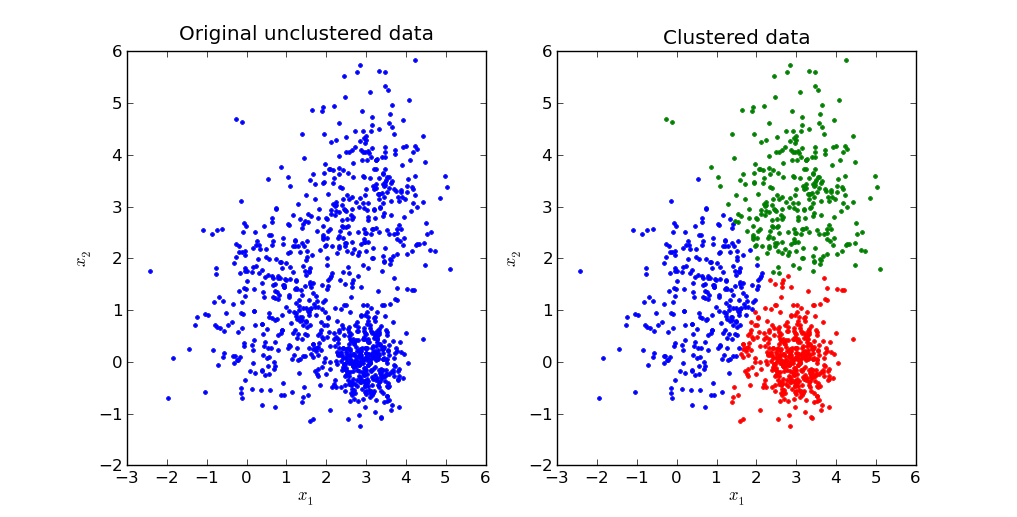
\includegraphics[width = 1.0 \textwidth]{Cluster.png}
         \caption{An example of clustering}
     \end{figure}
    \subsection{Maximum Likelihood Estimation}
    As the process of machine learning is to estimate a set of parameters �� based on observations of examples X, \textbf{maximum likelihood} is often considered the preferred estimator to use for machine learning.	

    \begin{itemize}
        \item Consider a set of $m$ examples $\mathbb X=\{\bm x^{(1)},...,\bm x^{(m)}\}$ drawn independently from the true but unknown data generating distribution $p_{data}(\bm x)$.
        \item Let $p_{model}(\bm x;\bm \theta)$ be a parametric family of probability distributions over the same space indexed by $\bm \theta$.
        \item The maximum likelihood estimator for $\bm \theta$ is then defined as 
            \begin{equation*}
                \begin{split}
                    \bm \theta_{ML} &= \arg \max_{\bm \theta}p_{model}(\mathbb X;\bm \theta) \\
                    &=\arg \max_{\bm \theta}\prod_{\bm x \in \mathbb X} p_{model}(\bm x;\bm \theta)\\
                    &=\arg \max_{\bm \theta}\sum_{\bm x \in \mathbb X} \log p_{model}(\bm x;\bm \theta)\\
                \end{split}
            \end{equation*}
    \end{itemize}

    \subsection{Input data}
    Previously observed data in the experience can be split to three categories:
    \begin{itemize}
        \item Training data: used to train the model
        \item Validation data: used to adjust the model
        \item Test data: used to evaluate the generalization of the model
    \end{itemize}
    Training data and validation data are usually splitted from a large observed data set. The ratio between training data and validation data is commenly 4:1 or 9:1.
    \subsection{Capacity and Performance}	

    The capacity of the learning algorithms can be under fitting, appropriate capacity and overfitting. Underfitting occurs when the model is not able to obtain a sufficiently low error value on the training set. Overfitting occurs when the gap between the training error and test error is too large.

    \begin{figure}[htbp]
        \centering
        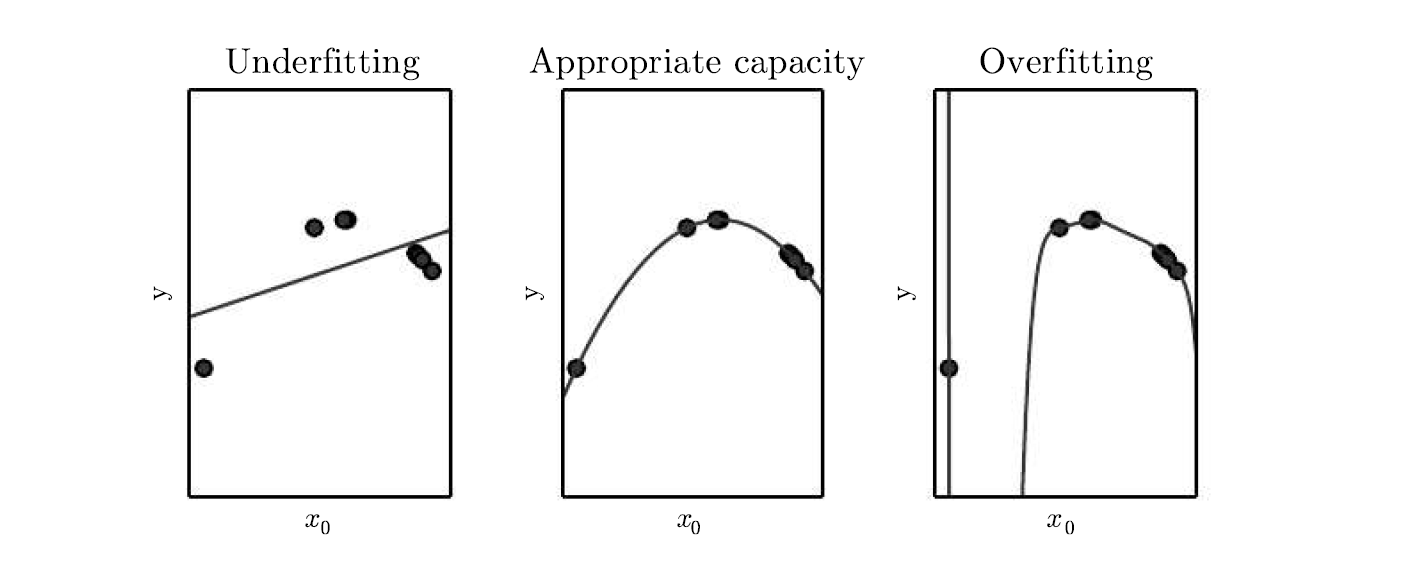
\includegraphics[width = 1.0 \textwidth]{fitCap.png}
        \caption{We fit three models to this example training set. The training data was
        generated synthetically, by randomly sampling $x$ values and choosing $y$ deterministically
        by evaluating a quadratic function. (Left)A linear function fit to the data suffers from underfitting-it cannot capture the curvature that is present in the data. (Center) A quadratic function fit to the data generalizes well to unseen points. It does not suffer from a significant amount of overfitting or underfitting. (Right)A polynomial of degree 9 fit to the data suffers from overfitting. Here we used the Moore-Penrose pseudoinverse to solve the underdetermined normal equations. The solution passes through all of the training points exactly, but we have not been lucky enough for it to extract the correct structure. It now has a deep valley in between two training points that does not appear in the true underlying function. It also increases sharply on the left side of the data, while the true function decreases in this area.}
    \end{figure}
    The factors determining the performance of the machine learning algorithms are:
    \begin{itemize}
        \item Test error (final error of the generated model) The error is calculated by a cost function based on the test data set
        \item The gap between training and validation error
    \end{itemize}
    The central challenge in machine learning is that we must perform well on new, previously unseen inputs, not just those on which our model was trained. So Machine learning algorithms indirectly minimize the test error. Regularization is the modification of machine learning algorithms to reduce validation error but not the training error in order to avoid overfitting.
    \begin{figure}[htbp]
        \centering
        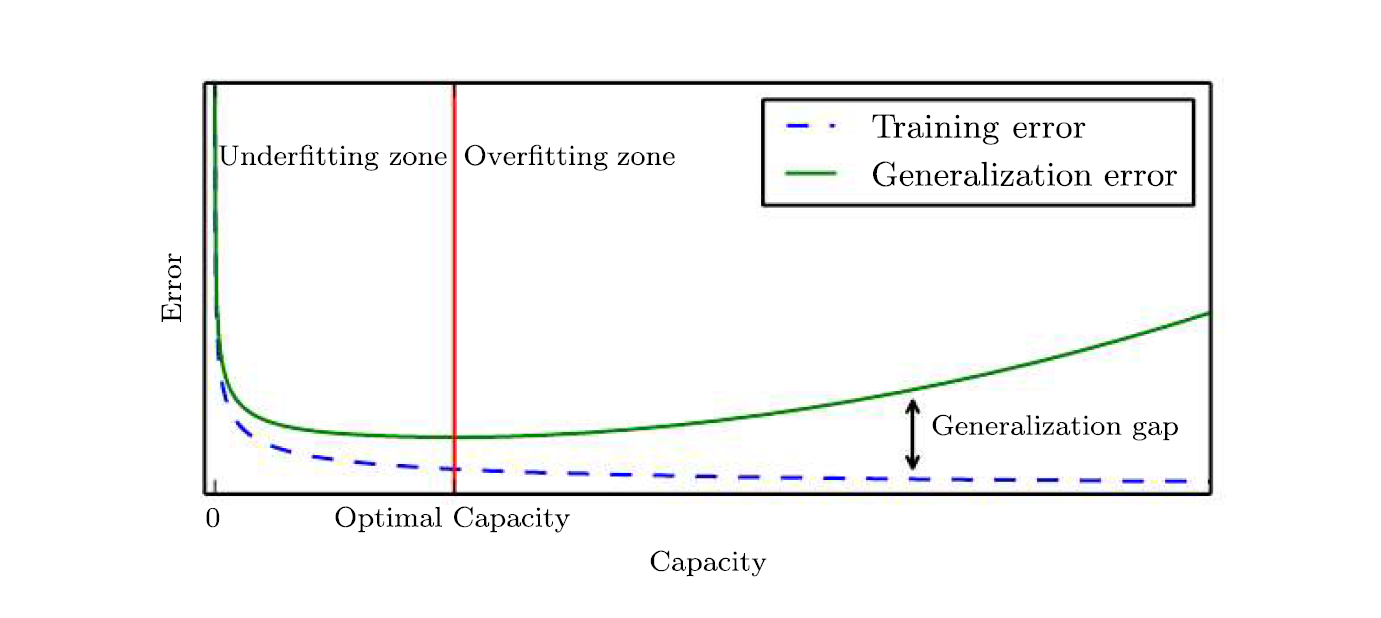
\includegraphics[width = 1.0 \textwidth]{ErrorwithCap.png}
        \caption{Typical relationship between capacity and error. Training and test error behave differently. At the left end of the graph, training error and generalization error are both high. This is the underfitting regime. As we increase capacity, training error decreases, but the gap between training and generalization error increases. Eventually, the size of this gap outweighs the decrease in training error, and we enter the overfitting regime, where capacity is too large, above the optimal capacity.}
    \end{figure}
    \section{Regularization and generalization}
    \subsection{Regularization}
    Regularization is a process of introducing additional information in order to prevent \textbf{overfitting}. Empirical learning of models (learning from a finite data set) is always an underdetermined problem, because in general we are trying to infer a function of any $x$ given only some examples $ x_{1},x_{2},...x_{n}$.

    A \textbf{regularization term} (or \textbf{regularizer}) $R(f)$ is added to a loss function:

    \begin{equation}
        \min _{f}\sum _{i=1}^{n}L(f({\hat {x}}_{i}),{\hat {y}}_{i})+\lambda R(f)
    \end{equation}

    where $L$ is an underlying loss function that describes the cost of predicting $ f(x)$ when the label is $y$ (for classification problem); and $\lambda$  is a parameter which controls the importance of the regularization term. $ R(f)$ is typically chosen to impose a penalty on the complexity of $f$. Concrete notions of complexity used include restrictions for smoothness and bounds on the vector space norm.

    \subsection{Generalization error}
    In supervised learning applications in machine learning and statistical learning theory, \textbf{generalization error} (also known as the \textbf{out-of-sample error}) is a measure of how accurately an algorithm is able to predict outcome values for previously unseen data. Because learning algorithms are evaluated on finite samples, the evaluation of a learning algorithm may be sensitive to sampling error. As a result, measurements of prediction error on the current data may not provide much information about predictive ability on new data. Generalization error can be minimized by \textbf{avoiding overfitting} in the learning algorithm.

    The generalization error, $I[f_{n}]$ of a particular function $f_{n}$ over all possible values of $x$ and $y$ is:

    \begin{equation}
        I[f_{n}]=\int _{X\times Y}V(f_{n}(x),y)\rho (x,y)dxdy
    \end{equation}
    Since $I[f_{n}]$ cannot be computed for an unknown probability distribution, the generalization error cannot be computed explicitly. Instead, the aim of many problems in statistical learning theory is to bound or characterize the generalization error in probability:
    \begin{equation}
        P_{G}=P(I[f_{n}]-I_{S}[f_{n}]\leq \epsilon )\geq 1-\delta _{n}
    \end{equation}
    while 
    \begin{equation}
        I_{S}[f_{n}]={\frac {1}{n}}\sum _{i=1}^{n}V(f_{n}(x_{i}),y_{i})
    \end{equation}
    is the empirical error computed from the sample points. 

    \section{Types of problems}
    \subsection{Classification problem}
    In machine learning and statistics, classification is the problem of identifying to which of a set of categories (sub-populations) a new observation belongs, on the basis of a training set of data containing observations (or instances) whose category membership is known. An example would be assigning a given email into "spam" or "non-spam" classes or assigning a diagnosis to a given patient as described by observed characteristics of the patient (gender, blood pressure, presence or absence of certain symptoms, etc.). 
     \begin{figure}[htbp]
         \centering
         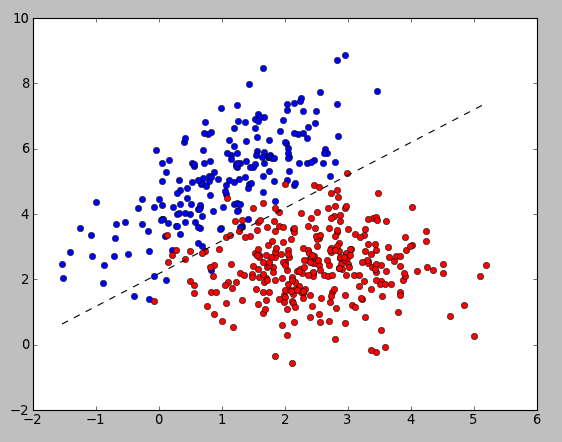
\includegraphics[width = 1.0 \textwidth]{Classification.png}
         \caption{An example of classification}
     \end{figure}
    \subsection{Regression problem}
    In statistical modeling, regression is a statistical process for estimating the relationships among variables. It includes many techniques for modeling and analyzing several variables, when the focus is on the relationship between a dependent variable and one or more independent variables (or 'predictors'). More specifically, regression analysis helps one understand how the typical value of the dependent variable (or 'criterion variable') changes when any one of the independent variables is varied, while the other independent variables are held fixed.  In all cases, the estimation target is a function of the independent variables called the \textbf{regression function}.
    \begin{figure}[htbp]
        \centering
        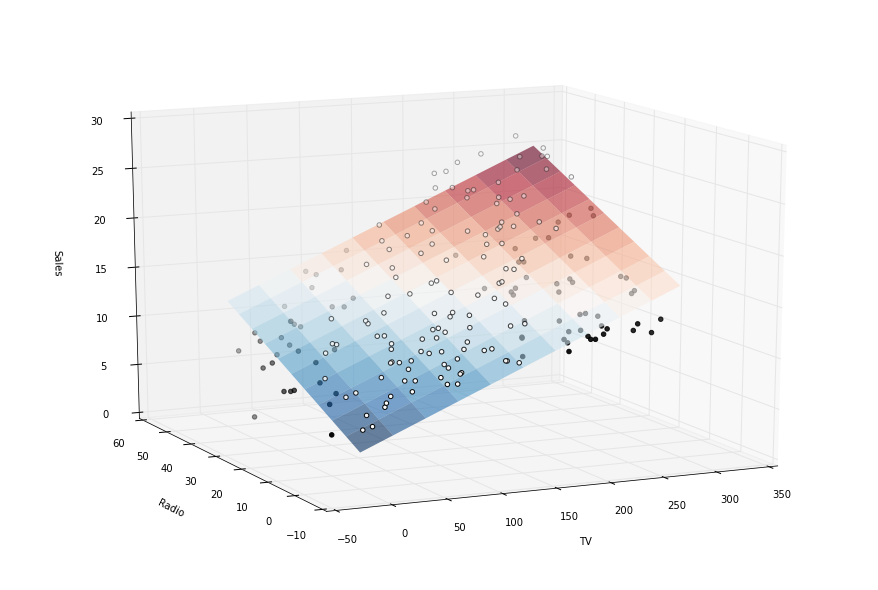
\includegraphics[width = 1.0 \textwidth]{Regression.png}
        \caption{An example of multivariate regression}
    \end{figure}


\section{Page Rank}
	\textbf{Page Rank} is a link analysis algorithm based on the Web graph (pages as nodes and hyper-links as edges), taking the rank value to indicate an importance of a particular page, which is defined recursively and	depends on the number of all pages that link to it (in-links).

	\subsection{The Simplest Model}
	The page in web can be regard as a node $A$ in a digraph $\mathcal G=(\mathcal V,\mathcal E)$. If the page $A$ have a hyper-link to page $B$, then there is a edge $A\rightarrow B$ in $\mathcal E$. For example, the web show in Figure \eqref{fig:fournodesweb} can be represented by a digraph $\mathcal G=(\mathcal V,\mathcal E)$ with
	\begin{gather*}
	\mathcal{V} =\{A,B,C,D\}\\
	\mathcal{E} =\{A\rightarrow B, A\rightarrow C,A\rightarrow D,B\rightarrow A,\\ B\rightarrow D,C\rightarrow A,D\rightarrow B,D\rightarrow C\}
	\end{gather*}
	\begin{figure}[h]
		\centering
		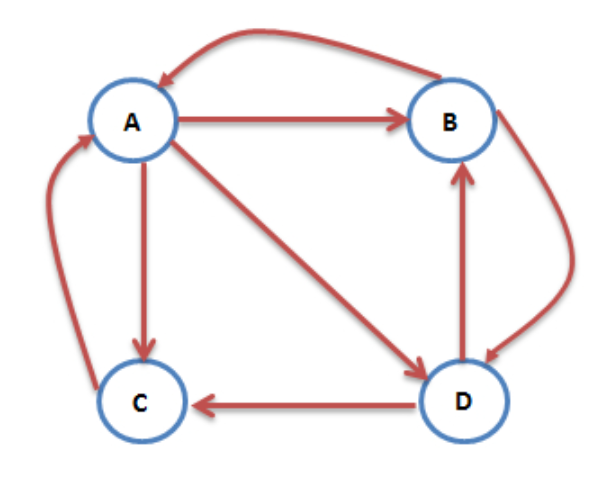
\includegraphics[width=0.7\linewidth]{fournodesweb}
		\caption{A web witch has 4 nodes}
		\label{fig:fournodesweb}
	\end{figure}
	
	Suppose there is a person Jack who is suffering the Internet, and at timing $t$, he is browsing page $A$. When he wants to leave page $A$, he will randomly click a hyper-link in page $A$ and go to browse next page and the possibility of clicking each page is the same. As an example in Figure \eqref{fig:fournodesweb}, each possibility from $A$ to $B,C,D$ are $\dfrac 13$. (If the page have no out-links, we can think it have a out-link to itself.) If we do that for each nodes, then we will have a transform matrix $M(\mathcal G)$. The transform matrix of the \eqref{fig:fournodesweb} is
	\begin{equation*}
		\begin{matrix}
		 to\backslash from&A&B&C&D\\
		A& &1/2 &1 &\\
		B&1/3 & & &1/2\\
		C&1/3 & & &1/2\\
		D&1/3 &1/2 & &
		\end{matrix}
	\end{equation*}
	i.e. 
	\begin{equation*}
	\mathbf M=\mathbf M(\mathcal{G})=
	\begin{pmatrix}
	 &1/2 &1 &\\
1/3 & & &1/2\\
1/3 & & &1/2\\
1/3 &1/2 & &
	\end{pmatrix}.
	\end{equation*}
	
	Now, we assume there are a large number of people, and at the timing $t=0$, each page has the same amount of people browsing it, i.e. for every page there are $\dfrac 1{|\mathcal V|}$ people browsing it at timing $t=0$. We use a vector $\mathbf v_0 =(\dfrac 1{|\mathcal V|},...,\dfrac 1{|\mathcal V|})^T$ to represent the initial state. 
	
	In the next timing $t=1$, every one randomly clicking a hyper-link in the page which he or she is browsing. Then the distribution of the people at $t=1$ is $$\mathbf v_1=\mathbf M\mathbf v_0.$$ By parity of reasoning, we can obtain the distribution of the people at $t=\mu$ is  $$\mathbf v_\mu=\mathbf M^\mu\mathbf v_0.$$
	
	We can regard this process is a Markov process, so the convergence of $\mathbf v_\mu$ is equivalent to the digraph $\mathcal G$ is \textbf{strongly connected}. So we have the following theorem:
	
	
	\begin{theorem}
		 $\mathbf v_\mu$ is convergent $\Leftrightarrow$ $\mathcal G$ is strongly connected
	\end{theorem}
	If we get the convergence result $\mathbf v_\infty$, the $i$th component $v_{\infty i}$ measures the importance of the $i$th page. Because the bigger $v_{\infty i}$ is, the more people will browse this page.
	Besides, by the theory of power method, we know if $\mathbf v_\mu$ is convergent, then the $\mathbf v_\infty$ is the corresponding eigenvector of the max eigenvalue of $\mathbf M$. 
	\subsection{More General Models}
	However the $\mathcal G$ of a real Internet web is impossible to be strongly connected, because there is always some pages have no out-links. Besides, if a page only have the out-link to itself, the result $\|\mathbf v_\infty\|$ may have no use value.
	
	Now we suppose Jack randomly click a hyper-link in the page with probability $\alpha$ or randomly input a new URL of a page with probability $1-\alpha$, so the iteration relation becomes:
	\begin{equation}\label{alpha}
	\mathbf v_{\mu+1}=(1-\alpha)\mathbf 1 +\alpha \mathbf M \mathbf v_\mu
	\end{equation}
	Because of $\|\mathbf v_0\|_1=1$ and the sum of each column of $\mathbf M$ is equal to 1, we can obtain $\|\mathbf v_\mu\|_1=1$ for any $\mu$. And the spectral radius of $\alpha \mathbf M$ is $$\rho(\alpha \mathbf M)=\alpha\rho(\mathbf M)\leq\alpha ||\mathbf M||_1=\alpha <1.$$ So the iteration \eqref{alpha} must be convergent, and $\mathbf v_\infty$ satisfy$$ 	\mathbf v_{\infty}=(1-\alpha)\mathbf 1 +\alpha \mathbf M \mathbf v_\infty.$$ 
	i.e.
	$$\mathbf v_\infty = (1-\alpha)(1-\alpha \mathbf M)^{-1}\mathbf 1 $$

